%% LyX 2.2.1 created this file.  For more info, see http://www.lyx.org/.
%% Do not edit unless you really know what you are doing.
\documentclass[english,headsepline,DIV=15,BCOR=0.125in,index=totoc,toc=listofnumbered,toc=graduated,unicode=true, twoside=true]{scrreprt}
\usepackage{amsmath}
\usepackage{amsthm}
\usepackage[libertine]{newtxmath}
\usepackage[T1]{fontenc}
\usepackage[latin9]{luainputenc}
\setcounter{secnumdepth}{3}
\setcounter{tocdepth}{3}
\usepackage{babel}
\usepackage{varioref}
\usepackage{textcomp}
\usepackage{graphicx}
\usepackage[unicode=true,
 bookmarks=true,bookmarksnumbered=false,bookmarksopen=false,
 breaklinks=false,pdfborder={0 0 0},pdfborderstyle={},backref=page,colorlinks=false]
 {hyperref}
\hypersetup{pdftitle={Oven Controller},
 pdfauthor={Robert Susmilch},
 pdfsubject={Domestic Oven Controller},
 pdfkeywords={Oven, domestic, stove, control, controller}}

\makeatletter

%%%%%%%%%%%%%%%%%%%%%%%%%%%%%% LyX specific LaTeX commands.
\newcommand{\noun}[1]{\textsc{#1}}

%%%%%%%%%%%%%%%%%%%%%%%%%%%%%% Textclass specific LaTeX commands.
 \newcommand{\callouttitleL}[1]{\def\callouttitleT{#1}}
 \newenvironment{callouttextL}
         {%
         ~\\[-0.25in]%
         \setlength\fboxsep{4pt}%
         \definecolor{shadecolor}{rgb}{1.00,0.90,0.90}%
         \begin{shaded}%
         \addtolength{\hsize}{-0.20\columnwidth}%
         {\centering\Large\callouttitleT\\[0.2cm]}%
         \noindent%
         \negmedspace{}%
         %\raggedright%
         %\setlength\parindent{16pt}%
 }%
 {%
         \end{shaded}%
         \par
 }%
                
\newenvironment{warningL}{\callouttitleL{Warning}\begin{callouttextL}}
                {\end{callouttextL}}
 \newenvironment{tipL}{\callouttitleL{Tip}\begin{callouttextL}}
 {\end{callouttextL}}

%%%%%%%%%%%%%%%%%%%%%%%%%%%%%% User specified LaTeX commands.
\KOMAoption{fontsize}{10pt}\recalctypearea
\usepackage{fontspec}

%\usepackage[osf,p,type1]{libertine}
\defaultfontfeatures{Ligatures = {Common, TeX}, Numbers = {Proportional, OldStyle, SlashedZero}, Contextuals = Swash, Fractions = On}% ,Scale=MatchLowercase} bug in current Biolinum
\setmainfont{Linux Libertine O}
\setsansfont{Linux Biolinum O}
\setmonofont[Numbers = {Monospaced, Lining, SlashedZero}]{Linux Libertine Mono O}
\usepackage[libertine]{newtxmath}

%\setromanfont [Ligatures={Common,TeX}, Numbers={OldStyle}]{Linux Libertine O}
%\setsansfont [Ligatures={Common}, BoldFont={Fontin Sans Bold}, ItalicFont={Fontin Sans Italic}]{Fontin Sans}
%\setsansfont[Ligatures={Common,TeX}, Numbers={OldStyle}]{Linux Biolinum O}
%\setromanfont [Ligatures={Common,TeX}, Numbers={OldStyle}]{Libertine}
%\setsansfont [Ligatures={Common}, BoldFont={Fontin Sans Bold}, ItalicFont={Fontin Sans Italic}]{Fontin Sans}
%\setsansfont[Ligatures={Common,TeX}, Numbers={OldStyle}]{Linux Biolinum O}

\usepackage[letterspace = 0, babel = true, protrusion = true, expansion = true]{microtype}
%\usepackage{textcomp}
%\usepackage{amsmath}
%\usepackage{amssymb}
\usepackage{lipsum}
\usepackage{lettrine}
\usepackage{minted}
\usepackage{tcolorbox}
\usepackage{etoolbox}
% Wrap minted environment in a pretty box.
\BeforeBeginEnvironment{minted}{\begin{tcolorbox}}%
\AfterEndEnvironment{minted}{\end{tcolorbox}}%
\setminted{breaklines,breakautoindent,autogobble,tabsize=2}
\newminted[asm]{nasm}{linenos, xleftmargin=1em}
\newminted[html]{html}{}
\newminted[java]{java}{}
\newminted[cpp]{cpp}{}
\newminted[make]{make}{}

\newcommand{\iasm}[1]{\mintinline{nasm}{#1}}

%\usepackage{enumitem}
%\setlist{nosep}
%\setlist{noitemsep} % to leave space around whole list
% More control per list
%\setlist[2]{noitemsep} % sets the itemsep and parsep for all level two lists to 0
%\setenumerate{noitemsep} % sets no itemsep for enumerate lists only
%\begin{enumerate}[noitemsep] % sets no itemsep for just this list
% ITEMS
%\end{enumerate}

\usepackage{mathdots}
\usepackage{url}

\usepackage{varioref}
\usepackage{hyperref}
\usepackage{cleveref}

\everymath{\displaystyle}

% Vertically stretch a table row this amount
%\renewcommand*\arraystretch{1.5}
% Or use this command
% \setlength{\extrarowheight}{2pt}


% Make nicer looking captions
%\usepackage{caption}
%\captionsetup{labelfont=bf,format=hang,justification=justified}

% Indent KOMA script captions
%\setcapindent{1em}

% Make KOMA script caption labels (eg Figure 1:) bold.
\addtokomafont{captionlabel}{\bfseries}

% Adjust the KOMA caption fonts smaller
%\setkomafont{caption}{\small\itshape}
\setkomafont{caption}{\small}
\setkomafont{captionlabel}{\usekomafont{caption}}
\usepackage{subfig}
%\captionsetup[subfloat]{font={footnotesize,it}}
\captionsetup[subfloat]{font={footnotesize}}


% Note that tables should have the caption above the table.
% Figures should have the caption below the table.
% Algorithms does not seem to matter above or below, though code above the caption looks nicer in LyX GUI
% Could adjust the caption spacing depending on the environment (document class)
%\captionsetup[table]{skip=20pt}
%\setlength{\abovecaptionskip}{15pt plus 10pt minus 2pt} % Chosen fairly arbitrarily

% Center figures and tables
\let\originaltable\table
\let\endoriginaltable\endtable
\renewenvironment{table}[1][ht]{%
\originaltable[#1]
\addfontfeatures{Numbers={Lining, Monospaced, SlashedZero}}
 \centering}%
{\endoriginaltable}

\let\originalfigure\figure
\let\endoriginalfigure\endfigure
\renewenvironment{figure}[1][ht]{%
\originalfigure[#1]
\centering}%
{\endoriginalfigure}

%\renewcommand*{\figureformat}{}
%\renewcommand*{\tableformat}{\tablename~\thetable}
%\renewcommand*{\captionformat}{}
\renewcommand*\thetable{%
%  \thechapter.%
  \@arabic\c@table
}

\renewcommand*\thefigure{%
%  \thechapter.%
  \@arabic\c@figure
}


% Force floats to appear in their respective sections, subsections, and subsubsections.
%\usepackage[section,subsection,subsubsection]{extraplaceins}
\usepackage[section, subsection]{extraplaceins}

%\makeatletter
\if@twoside % commands below work only for twoside option of \documentclass
    \newlength{\textblockoffset}
    \setlength{\textblockoffset}{12mm}
    \addtolength{\hoffset}{\textblockoffset}
    \addtolength{\evensidemargin}{-2.0\textblockoffset}
\fi
%\makeatother
\title{Oven Controller}
\author{Robert Susmilch}
\usepackage{scrlayer-scrpage}
\pagestyle{scrheadings}
%\makeatletter
\let\papertitle\@title
\let\paperauthor\@author
\let\paperdate\@date
%\makeatother
\lehead[\papertitle]{\papertitle}
\rehead[\paperauthor]{\paperauthor}
\lohead[\paperauthor]{\paperauthor}
\rohead[\papertitle]{\papertitle}

\definecolor{green}{RGB}{0, 180, 0}
%\definecolor{cyan}{RGB}{0, 180, 180}
\definecolor{blue}{RGB}{0,100,255}
\definecolor{yellow}{RGB}{200,200,0}
\definecolor{Black}{RGB}{0, 0, 0}
\definecolor{Gray}{RGB}{150, 150, 150}
\definecolor{teal}{RGB}{64, 128, 128}
\definecolor{gray}{rgb}{0.95,0.95,0.95}
\definecolor{muave}{rgb}{0.58,0,0.82}

\usepackage{framed}

\usepackage{xcolor}% http://ctan.org/pkg/xcolor
\newcommand{\myquote}[2][black!10]{%
  \medskip
  {\setlength{\fboxsep}{.1\columnwidth}%
  \noindent\colorbox{#1}{\begin{minipage}{\dimexpr\columnwidth-2\fboxsep}
    \raggedright\sffamily\bfseries\Huge#2
  \end{minipage}}} \par
  \medskip
}
%\newcommand{\hltt}[1]{\textcolor{blue}{#1}}
%\usepackage{footnote}
\setminted{breaklines,breakautoindent,autogobble,tabsize=2}
\newminted[bash]{bash}{}

% Use to include text files into a LaTeX file, such as source files
\usepackage{fancyvrb}
% redefine \VerbatimInput
\RecustomVerbatimCommand{\VerbatimInput}{VerbatimInput}%
{fontsize=\footnotesize,
 %
 frame=lines,  % top and bottom rule only
 framesep=2em, % separation between frame and text
 rulecolor=\color{Gray},
%
 label=\fbox{\color{Black}Passwords},
 labelposition=topline,
 %
 %commandchars=\|\(\), % escape character and argument delimiters for
                      % commands within the verbatim
 commentchar=*        % comment character
}
% Then we use
%\VerbatimInput{yourFileInSameDirectory.txt}

\usepackage{enumitem}
\setlist[itemize,1]{label=$\bullet$}
\setlist[itemize,2]{label=\tiny$\blacklozenge$}
\setlist[itemize,3]{label=\tiny$\blacktriangleright$}
\setlist[itemize,4]{label=\tiny$\blacksquare$}
\setlist[itemize,5]{label=$\circ$}
\setlist[itemize,6]{label=$\triangleright$}
\setlist[itemize,7]{label=$\star$}
\setlist[itemize,8]{label=$\ast$}
\setlist[itemize,9]{label=$\star$}

\renewlist{itemize}{itemize}{9}
\setlist[itemize]{noitemsep}

% KOMA script won't include the nomenclature within the table of contents
\def\nompreamble{\addcontentsline{toc}{section}{\nomname}\markboth{\nomname}{\nomname}}
%\DeclareUnicodeCharacter{21AA}{\hookarrow}

% Highlight nomenclature terms in some way.
\newcommand{\term}[1]{\textcolor{blue}{#1}}
%\newcommand{\term}[1]{\texttt{#1}}
\newcommand{\code}[1]{\texttt{#1}}
\newcommand{\tn}[1]{\term{\noun{#1}}}

\usepackage{listings}

\lstdefinelanguage{ijvm}
{morekeywords={BIPUSH, DUP, GOTO, IADD, IAND, IFEQ, IFLT, IF\_ICMPEQ, IINC, ILOAD, INVOKEVIRTUAL, IOR, IRETURN, ISTORE, ISUB, LDC\_W, NOP, POP, SWAP, WIDE, RD, WR, FETCH, if},
sensitive = false,
morecomment=[l]{//},
emph={A, B, N, Z, MDR, PC, MBR, MBRU, SP, LV, CPP, TOS, OPC, MPC},
emph={[2]H, MAR},
emphstyle={\color{blue}},
emphstyle={[2]\color{muave}}
}

\lstdefinelanguage{arm}
{morekeywords={add, cmp, blt,mov},
sensitive = false,
morecomment=[l]{;},
emph={R0, R1, R2, R3, R4, R5, R6},
emph={[2]H, MAR},
emphstyle={\color{red}},
emphstyle={[2]\color{muave}}
}

\lstset{%
language=ijvm,
basicstyle={\ttfamily},
breaklines=true,
commentstyle={\color{teal}\textit},
keywordstyle={\color{blue}},
rulecolor={\color{black}},
backgroundcolor={\color{gray}},
stringstyle={\color{muave}},
frame=single,
numbers=left,
numberstyle={\scriptsize}}

\newcommand{\ijvm}[1]{\lstinline[language=ijvm]{#1}}
\usepackage[maxfloats=25]{morefloats}
\widowpenalty=10000
\clubpenalty=10000 

\makeatother

\begin{document}

\title{Oven Controller}

\subtitle{User Manual}

\titlehead{Copyright � 2016 Robert Susmilch}

\author{Robert Susmilch}

\date{September 3, 2016}

\maketitle
\tableofcontents{}

%\cleardoublepage\null

\cleardoublepage{}

\setcounter{chapter}{1}

\chapter{Overview}

\section{Basics}

The user interface is composed of an \noun{led} display with integrated
buttons. The button functions are as shown in \vref{fig:Primary-user-interface_buttons}.
The 8-segment numerical display outputs various information, such
as current oven mode, timer count down and control inputs. The \noun{led}s
above the buttons and below the 8-segment display are status indicators
for various oven modes and functions (see \vref{fig:Primary-user-interface_status_LEDs}.)

A secondary 8-segment \noun{led} display is included that allows longer
length user messages (such as error and alarm output) as well as supplements
various oven functions. Typically the secondary display outputs the
current oven temperature as well as the current oven bake or broil
set temperature. Alternatively, the display can be set to output the
current control board's temperature and the current oven temperature.
This alternative output mode can be easily determined due to the first
display temperature having all decimal points lit.

\begin{figure}
\noindent \begin{centering}
\includegraphics[width=0.9\columnwidth]{\string"Controller Off_Buttons\string".png}
\par\end{centering}
\caption{Primary user interface display. Buttons are as labeled.\label{fig:Primary-user-interface_buttons}}

\end{figure}

\begin{figure}
\noindent \begin{centering}
\includegraphics[width=0.9\columnwidth]{\string"Controller Off_Status\string".png}
\par\end{centering}
\caption{Primary user interface with status \noun{led}s labeled.\label{fig:Primary-user-interface_status_LEDs}}

\end{figure}

\begin{figure}
\caption{Secondary display used for oven temperatures.}

\end{figure}


\section{Control}

\subsection{Power Up}

During initial power up (such as after plugging in or turning on the
electric panel breaker) the oven controller will display a welcome
message, and proceed to test output functions by illuminating all
\noun{led} segments and sounding the alert beeper. The oven will then
enter standby mode.

\subsection{Modes}

The oven has the following modes:
\begin{itemize}
\item Standby
\begin{itemize}
\item Standby mode indicates the oven is not currently heating, tracking
a timer and that the clock has not been set.
\item There is \emph{no} status \noun{led} indicating standby mode.
\begin{itemize}
\item Indicated by the display output of ``standby'' (\vref{fig:Standby-mode})
or, if the clock is set, showing the current time with the status
\noun{led}s slowly counting up (in binary fashion.)
\end{itemize}
\item If oven was previously on, the temperature indicated by the secondary
display should slowly decline.
\end{itemize}
\end{itemize}
\begin{figure}
\noindent \begin{centering}
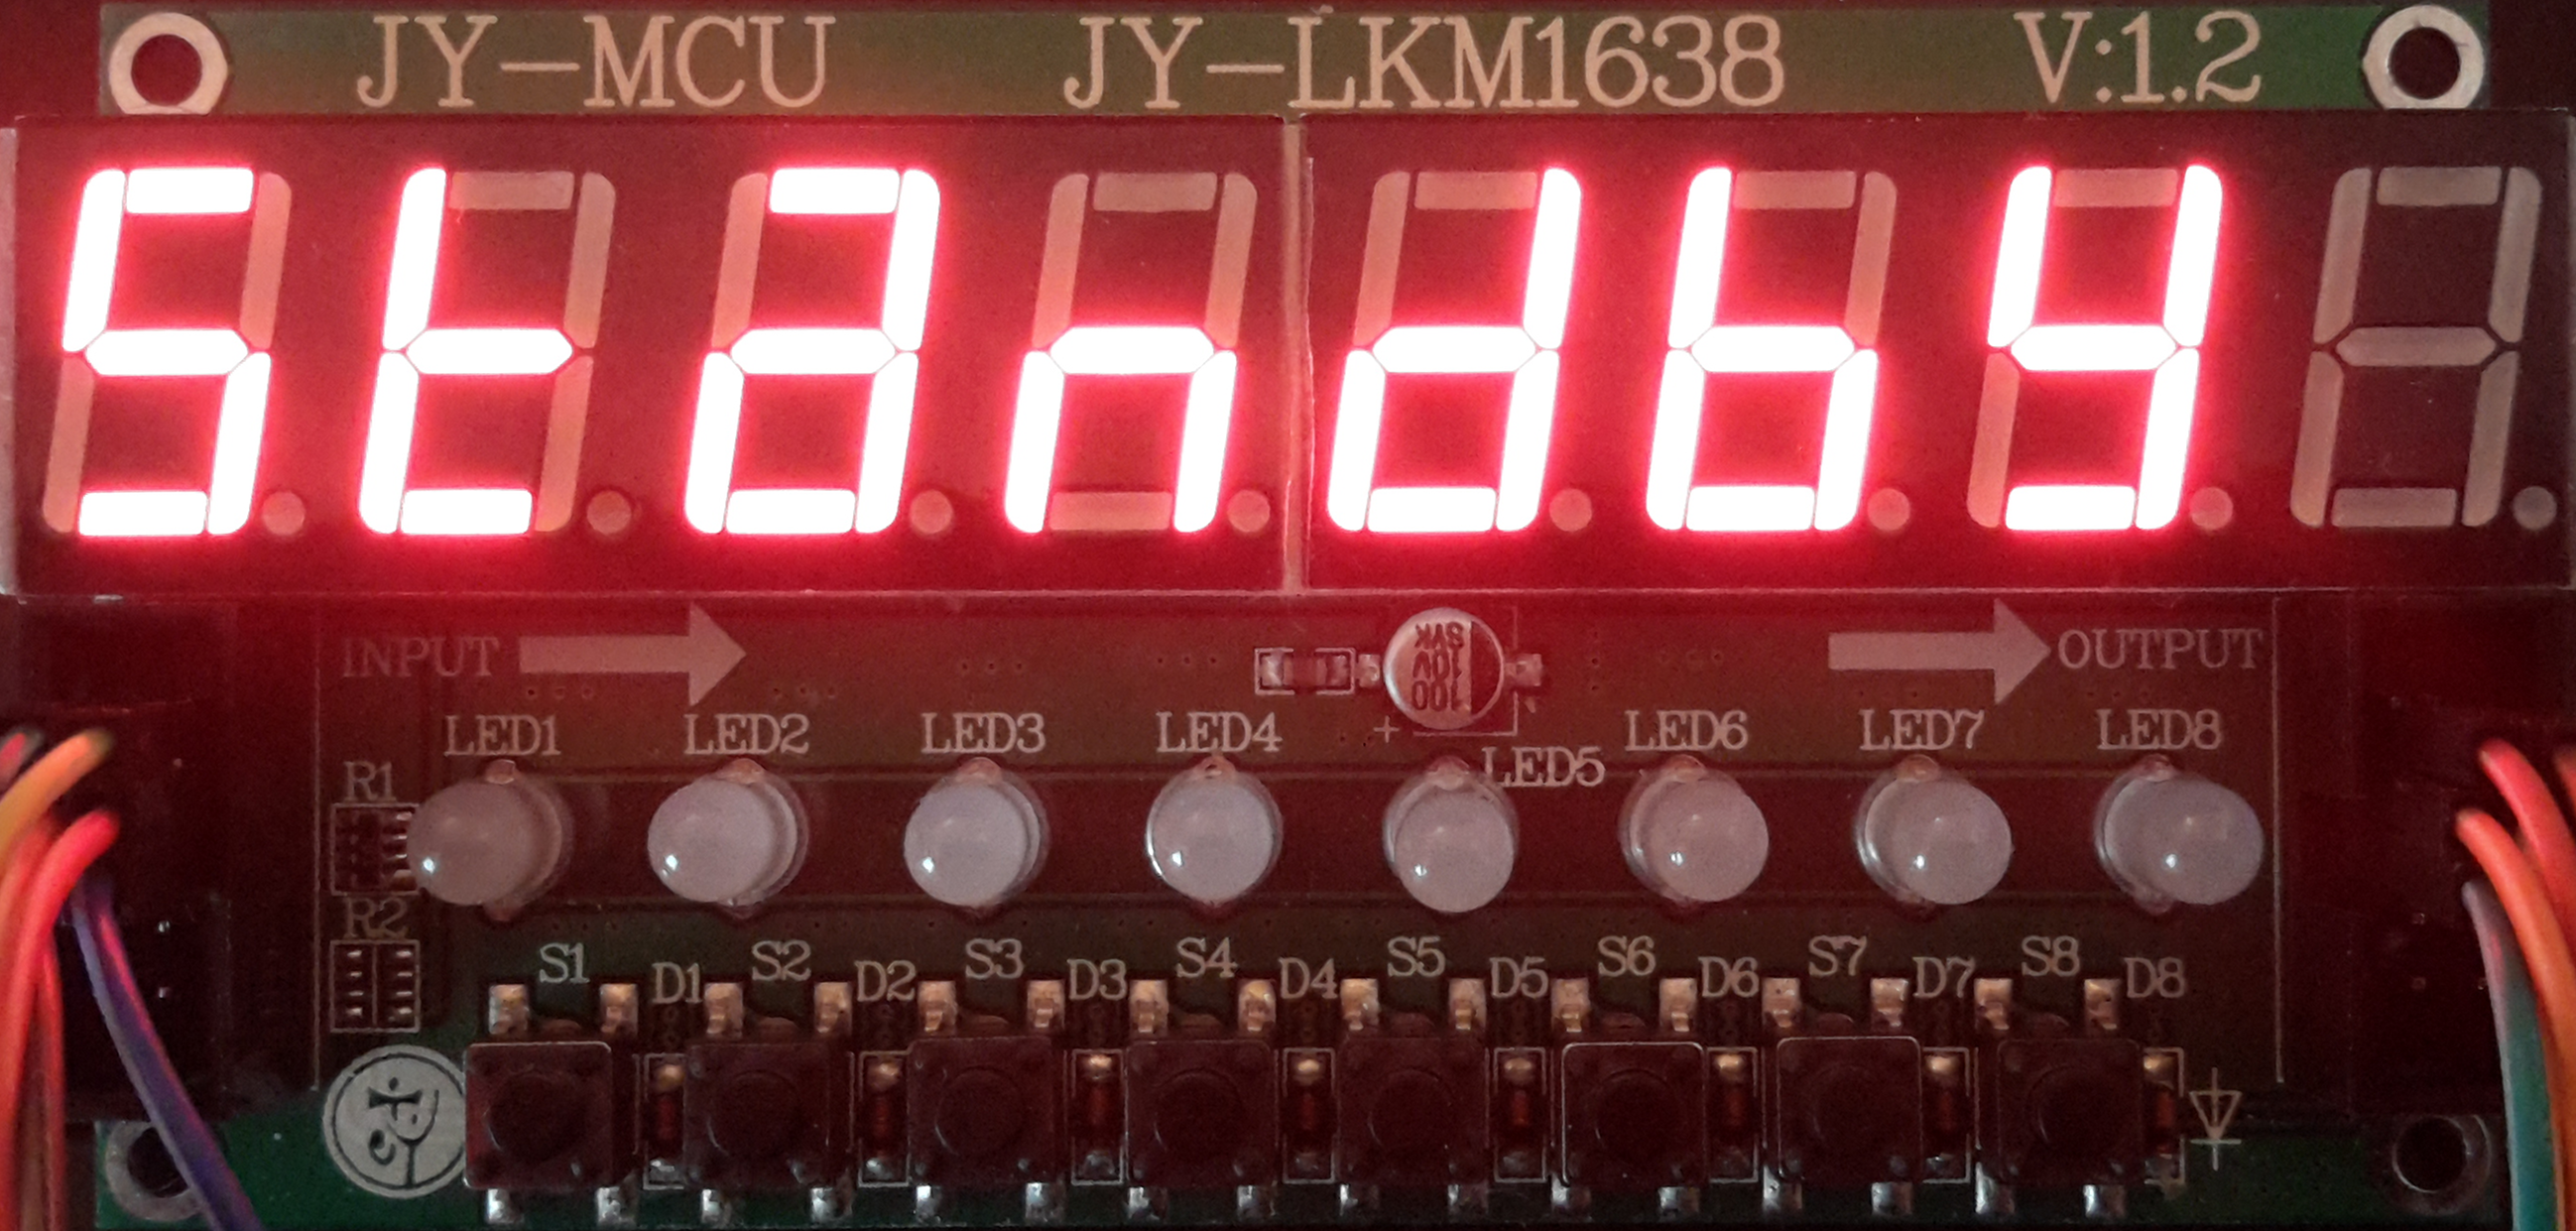
\includegraphics[width=0.9\columnwidth]{Standby}
\par\end{centering}
\caption{Standby mode is when the oven is currently not preforming a task,
in other words it is idle awaiting a command.\label{fig:Standby-mode}}

\end{figure}

\begin{itemize}
\item Timer
\begin{itemize}
\item Timer mode allows tracking time
\begin{itemize}
\item Depends on whether oven is currently on
\begin{itemize}
\item If oven is not in bake or broil mode, timer mode functions as a traditional
kitchen timer.
\item If oven is currently in bake or broil mode, the timer will \emph{automatically}
turn off the oven when the timer expires.
\end{itemize}
\end{itemize}
\item Timer mode is indicated by the ``timer'' status \noun{led} and a
decreasing time display.
\end{itemize}
\item Bake / broil
\begin{itemize}
\item Bake mode is for normal oven baking.
\begin{itemize}
\item During bake preheat \emph{both} oven elements (bake and broil) are
used to quickly and evenly heat the oven.
\item Bake mode occasionally cycles the broil element on to help even out
cooking.
\end{itemize}
\item Broil mode utilizes \emph{only} the broil element, both during preheat
and normal broil operation.
\item Status \noun{led}s
\begin{itemize}
\item Bake mode is indicated by the ``bake'' status \noun{led}.
\item Broil mode is indicated by the ``broil'' status \noun{led}.
\end{itemize}
\item Once a temperature is entered the oven will heat to the set temperature
and cycle the bake and broil elements on and off.\footnote{There is an automatic safety timer. Please see the oven temperature
section.}
\end{itemize}
\item Clock
\begin{itemize}
\item If the clock time is set, during standby the display will show the
current time.
\item Times are set in 24 hour mode (military time.)
\item The clock function does not utilize a battery backup, and will lose
the time if power is lost.
\begin{itemize}
\item If power is lost, the controller will not display the clock during
standby. Instead the display will simply state ``standby'' indicating
the oven is idle.
\end{itemize}
\end{itemize}
\end{itemize}

\subsection{Operation}

Please see \vref{fig:Primary-user-interface_buttons} for button locations,
and \vref{fig:Primary-user-interface_status_LEDs} for status \noun{led}s.

\subsubsection{Bake}

\paragraph{Entering a bake temperature}
\begin{itemize}
\item Bake mode can be entered by pressing the ``bake button.''
\begin{itemize}
\item The ``bake'' status\noun{ led} will light by itself to signify the
user is in the bake setting menu.
\item The display will change to show the set temperature the user desires
for the oven.
\item See \vref{fig:Oven_temp_setting}.
\end{itemize}
\item The user may press, or hold the up and down buttons to enter the desired
temperature.
\item Once the desired temperature is displayed, pressing enter will start
the bake mode.
\begin{itemize}
\item The display will flash the status \noun{led}s to indicate acknowledgment
of the users entry.
\item If the oven was \emph{not previously} in a bake or broil mode, the
oven will now enter preheat mode.
\begin{itemize}
\item Display will state ``preheat''\footnote{Unless the timer function is already active.}
and the ``preheat'' \noun{led} will light.
\end{itemize}
\item If the oven was already in bake or broil mode, the oven will \emph{not}
preheat, and instead follow the normal thermostat setting.
\end{itemize}
\end{itemize}
\begin{warningL}
Preheat mode utilizes \emph{both} oven elements to quickly heat the
oven. Due to the extended times required to heat a cold oven, and
the fact that the broil element will be on, food placed inside the
oven before the preheat cycle is done will burn.
\end{warningL}

\begin{figure}
\includegraphics[width=0.9\columnwidth]{\string"Temp Setting\string".png}

\caption{Display of the bake temperature setting menu. We note the current
temperature setting is 100\textdegree F and that the ``bake'' \noun{led}
status light is lit.\label{fig:Oven_temp_setting}}
\end{figure}

\begin{itemize}
\item The status \textsf{\noun{led}}s\textsf{ will show that the ``bake''
}\noun{led} is lit, signifying that the oven is in bake mode.
\item \textsf{The} secondary display will show the set point temperature
(or internal board temperature) and current oven temperature (see
\vref{fig:Secondary-display-oven_temp}.)
\item The oven will \emph{automatically} enter a safety timer to prevent
leaving the oven on for long periods unattended. See important notice
regarding the mandatory timer.
\end{itemize}
\begin{figure}
\noindent \begin{centering}
\includegraphics[width=0.9\columnwidth]{\string"Oven Temp\string".png}
\par\end{centering}
\caption{Secondary display showing internal (board) temperature (73\textdegree F,
indicted by three decimal points) and current oven temperature (71\textdegree F).\label{fig:Secondary-display-oven_temp}}
\end{figure}


\callouttitleL{Mandatory Preheat Timer}
\begin{callouttextL}
Once preheat mode is entered, an automatic safety timer of 20 minutes
is started to reach oven set point temperature. If the oven does not
reach the set temperature in that time frame the timer alarm will
sound and the oven will shut off.

Additionally, once the oven reaches the desired temperature, the safety
timer is reset to 20 minutes and the oven will shut down \textbf{unless}
the user enters a time using the timer function.

Once a timer has been started, the mandatory timer is deactivated
and the stove will heat until the user supplied timer is exhausted.
\end{callouttextL}

\begin{warningL}
\textbf{Do not} attempt to bypass or deactivate the mandatory safety
timer. Ovens and stoves are the \emph{number one} cause of household
fires and unattended cooking is a safety hazard.

Do not rely on the mandatory timer to turn off the oven. \textbf{Always}
shutdown and \textbf{confirm} the oven is off, the status \noun{led}s
indict no heating modes, the ``warm'' status \noun{led} is off and
that the temperature is approximately at \textbf{ambient} (room) temperature
before leaving the oven unattended.
\end{warningL}


\subsubsection{Preheat}
\begin{itemize}
\item If the oven is in preheat mode, once the oven reaches the entered
temperature, the preheat alarm will sound.
\begin{itemize}
\item The oven will beep and flash the status \noun{led}s to let the user
know the oven has reached temperature.
\item The preheat alarm can be canceled by pressing any button.
\item The user is encouraged to enter a time into the oven timer to avoid
automatic oven shutdown due to the mandatory timer.
\end{itemize}
\end{itemize}
\begin{tipL}
Always remember to enter a timer when cooking to prevent automatic
shutdown.
\end{tipL}


\subsubsection{Broil}
\begin{itemize}
\item Broil mode operates in the same manner as bake mode.
\begin{itemize}
\item The bake element is never used during heating.
\item There is no preheat mode.
\end{itemize}
\item All operations function similarly, including the mandatory safety
timer.
\end{itemize}

\subsubsection{Canceling or turning off the oven}
\begin{itemize}
\item To turn off the oven in either bake or broil modes, press the appropriate
button (bake if baking, broil if broiling) and \emph{again} press
the same button to cancel that mode.
\begin{itemize}
\item The display will flash and the appropriate bake or broil status \noun{led}
will go out.
\end{itemize}
\end{itemize}

\subsubsection{Timer}
\begin{enumerate}
\item Pressing the ``timer'' button will enter the timer setting menu.
\begin{enumerate}
\item The timer status \noun{led} will light alone to signify one is in
the timer menu.
\end{enumerate}
\item The display will show ``Hr'' signifying that the user is now entering
the number of hours required (\vref{fig:Timer-entry-hours}.)
\begin{enumerate}
\item The hour decimal point will flash as well to additionally confirm
entry.
\end{enumerate}
\item Using the up and down buttons enter the required number of hours.
\item Pressing enter confirms the number of hours.
\item The display will now show ``Min'' to signify entering minutes (\vref{fig:Timer-entry-minute}.)
\begin{enumerate}
\item The minute decimal point will flash to confirm minutes are being entered.
\end{enumerate}
\item Pressing enter a second time confirms the time and starts the timer.
\begin{enumerate}
\item The status \noun{led}s will flash and the display will now show the
countdown timer.
\item The ``timer'' status \noun{led} will now be lit, indicating a timer
is running.
\end{enumerate}
\item When the timer is exhausted, the controller will enter an alarm state.
\begin{enumerate}
\item The display will show ``timer.''
\item A status \noun{led}s will flash and a beeper will sound indicting
that the timer has expired.
\item If the oven is currently in bake or broil mode, \emph{the oven will
shutdown.}
\end{enumerate}
\end{enumerate}
\begin{tipL}
When the timer expires while cooking in the oven, the oven will \emph{automatically}
shutdown. This helps to prevent over cooking or burning of food.
\end{tipL}

\begin{figure}
\noindent \begin{centering}
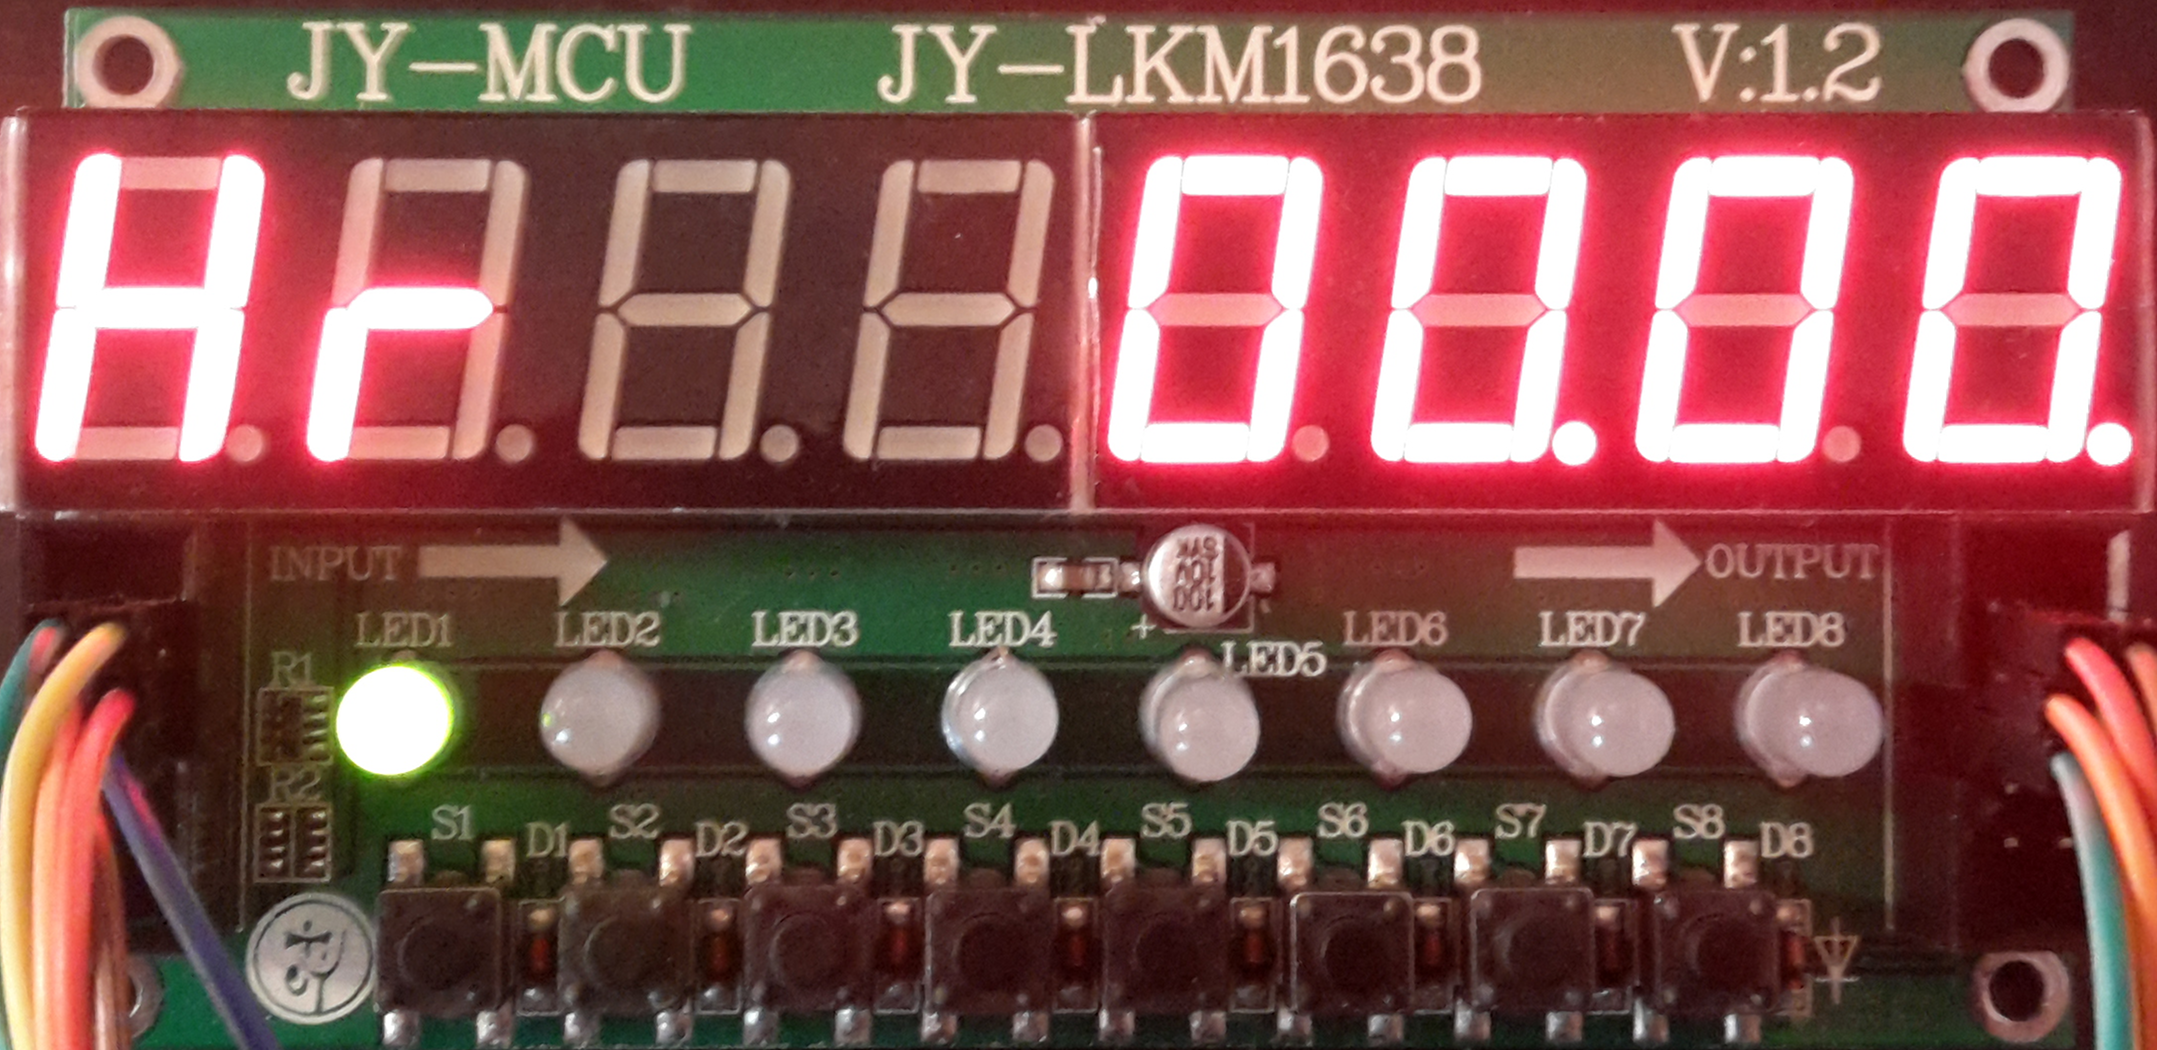
\includegraphics[width=0.9\columnwidth]{Hour}
\par\end{centering}
\caption{Timer entry showing prompt for desired number of hours.\label{fig:Timer-entry-hours}}

\end{figure}

\begin{figure}
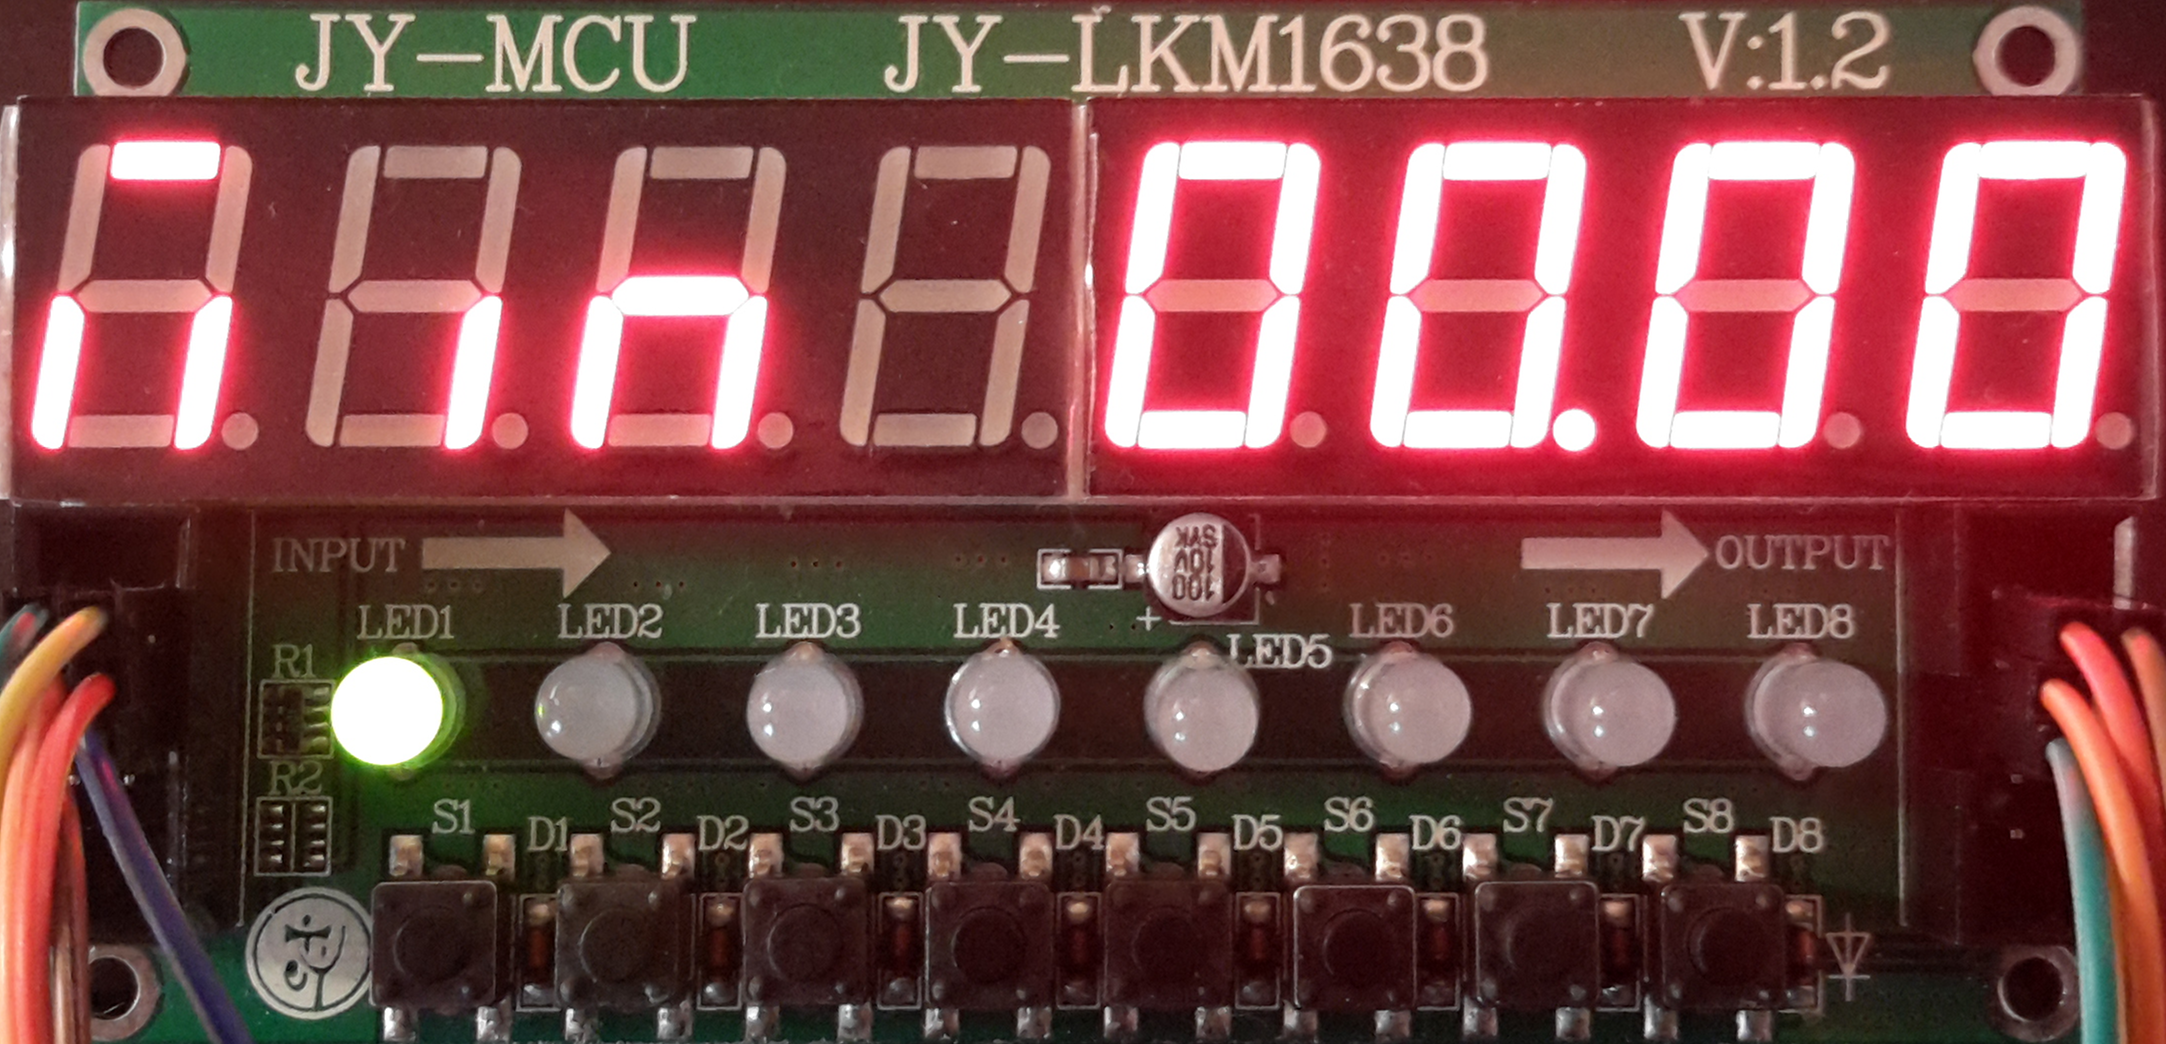
\includegraphics[width=0.9\columnwidth]{Minute}

\caption{Timer entry showing prompt for desired number of minutes. The unusual
``M'' is due to the limited possibilities for character display
on 8-segment \noun{led}s.\label{fig:Timer-entry-minute}}

\end{figure}


\subsubsection{Exiting a menu}
\begin{itemize}
\item To cancel entering a temperature or time press the ``cancel / back.''
\item Additionally, if no button is pressed for approximately 10 seconds,
the controller will automatically cancel and exit the temperature
menu.
\end{itemize}
\begin{tipL}
Pressing ``back'' or allowing the menu to time out, \emph{will not}
cancel the appropriate oven function (such as turning off a timer
or shutting off the oven.) Canceling the setting menu will simply
\emph{exit} the menu without changing any settings. The oven will
continue to operate in any modes it was currently in, such as baking
or timing.
\end{tipL}


\end{document}
